%%%%%%%%%%%%%%%%%%%%%%%%%%%%%%%%%%%%%%%%%
% Beamer Presentation
% LaTeX Template
% Version 1.0 (10/11/12)
%
% This template has been downloaded from:
% http://www.LaTeXTemplates.com
%
% License:
% CC BY-NC-SA 3.0 (http://creativecommons.org/licenses/by-nc-sa/3.0/)
%
%%%%%%%%%%%%%%%%%%%%%%%%%%%%%%%%%%%%%%%%%

%----------------------------------------------------------------------------------------
%	PACKAGES AND THEMES
%----------------------------------------------------------------------------------------

\documentclass{beamer}

\mode<presentation> {
	\usetheme{Madrid}
%\usetheme{Boadilla}
%\usetheme{Antibes}
%\usetheme{JuanLesPins}

	%\setbeamertemplate{footline} % To remove the footer line in all slides uncomment this line
	%\setbeamertemplate{footline}[page number] % To replace the footer line in all slides with a simple slide count uncomment this line
	
	%\setbeamertemplate{navigation symbols}{} % To remove the navigation symbols from the bottom of all slides uncomment this line
	
	%\addtobeamertemplate{frametitle}{}{\section{\insertframetitle}} % To add all frame title into table of contents automacitally
	
	%\setbeamertemplate{items}[square]
}

\usepackage{graphicx}
\usepackage{booktabs} % Allows the use of \toprule, \midrule and \bottomrule in tables


%----------------------------------------------------------------------------------------
%	TITLE PAGE
%----------------------------------------------------------------------------------------

\title[DragonFly]{Project DragonFly \\ Surveil Transport sector into Smart City}
\author[Group 3]{
	{\small \textbf{\textit{Group 3}}} \\
	Abhinand C \\
	Edwin Jose George \\
	Lavanya E.V \\
	Shilpa Suresh \\
	\medskip
	{\small \textit{Guided by:}} Dr. Rafeeque P.C \\
}
\institute[GCEK]{Department of Computer Science and Engineering \\
	Government College of Engineering Kannur
}
\date{\today}

\begin{document}

\begin{frame}
\titlepage
\end{frame}

\begin{frame}
\frametitle{Contents}
\tableofcontents
\end{frame}

%########################################################################################
%	PRESENTATION SLIDES
%########################################################################################

\section{Introduction}
\begin{frame}{Introduction}
    
    \begin{itemize}
    	\item Increased accessibility of road transportation system massively increase in road traffic, carbon dioxide emissions, road accident risks.
    	
    	\item Traffic management authorities faces hectic challenges to maintain an undisturbed transportation
system. (tracking the suspicious vehicle, handling traffic jam etc)
    	
    	\item The wide gap in human resource availability and the tedious effort required for traffic analysis (very huge data).
    \end{itemize}
\end{frame}


%########################################################################################

\section{Motivation}
\begin{frame}{Motivation}
	\begin{itemize}
		\item Current system make use of manual approach of reviewing long video clips to identify the suspect vehicle. Various possible routes that can be taken by suspect further makes the process of re-identification very difficult and time consuming.
		
		\item There do not exist an approachable system where user can interact via simple textual description to lookup suspect vehicles.
		
		\item Traffic flow analysis can aid in Anomaly detection, Alert Control System, \& emergency services.		
	\end{itemize}
	
\end{frame}

%########################################################################################

\section{Literature Review}
\begin{frame}{Literature Review}
\begin{table}[!h]
	\centering
	\resizebox{\textwidth}{!}{%
		\begin{tabular}{|l|l|l|l|}
			\hline
			\multicolumn{1}{|c|}{\textit{\textbf{Title}}} &
			\multicolumn{1}{c|}{\textit{\textbf{Method}}} &
			\multicolumn{1}{c|}{\textit{\textbf{Pros and Cons}}} &
			\multicolumn{1}{c|}{\textit{\textbf{Challenges}}} \\ \hline
			\begin{tabular}[c]{@{}l@{}}CityFlow: A City-Scale \\ Benchmark for Multi-Target\\ Multi-Camera  Vehicle\\  Tracking and  \\ Re-Identification\end{tabular} &
			\begin{tabular}[c]{@{}l@{}}Use of Multi-Target Single Camera\\ and Multi-Target Multi-Camera \\ tracking.\\ \\ Use visual-spatio-temporal\\ reasoning\end{tabular} &
			\begin{tabular}[c]{@{}l@{}}Pros:\\ Better and faster results.,\\ Handle large scale recognition\\ Tracking and small prediction\\ \\ Cons:\\ Overlapping viewpoints,\\ Implemented only at junction \\ points\end{tabular} &
			\begin{tabular}[c]{@{}l@{}}High quality videos\\ \\ Multiple viewpoints on \\ same object\\ \\ Require annotated videos\end{tabular} \\ \hline
			\begin{tabular}[c]{@{}l@{}}Real-Time Vehicle Make and\\ Model Recognition System\end{tabular} &
			\begin{tabular}[c]{@{}l@{}}Random Forest and Support Vector\\  Machine coupled with traditional\\ Vehicle Make Model Recognition\\ System,\\ \\ Usage of Histogram of Oriented \\ Gradient (HOG) and GIST \\ features\end{tabular} &
			\begin{tabular}[c]{@{}l@{}}Pros:\\ Superior processing speed \& \\ recognition accuracy wrt existing \\ VMMR, Accounts for partial \\ viewpoints\\ \\ Cons:\\ High dimensional,  Region of \\ interest is only on parts, No global\\  representation\end{tabular} &
			\begin{tabular}[c]{@{}l@{}}Computational time increases\\ with increase of blocks HOG\\ \\ Limited Region of Interest\end{tabular} \\ \hline
			\begin{tabular}[c]{@{}l@{}}Efficient and Deep Vehicle \\ Re-Identification Using \\ Multi-Level Feature \\ Extraction\end{tabular} &
			\begin{tabular}[c]{@{}l@{}}Global channel extracts single \\ feature generalizing whole image,\\ \\ Local channel extract multiple\\  local features (logo, stickers),\\ \\ Attribute channel extracts \\ color, model, type\end{tabular} &
			\begin{tabular}[c]{@{}l@{}}Pros:\\ Extraction of inter and intra features,\\ Data augmentation with license plate \\ verification\\ \\ Cons:\\ Requires Data augmentation,\\ Effected by illuminations\end{tabular} &
			\begin{tabular}[c]{@{}l@{}}Cross camera vehicle tracking\\ \\ Changes in color response\\ \\ Background clutter\end{tabular} \\ \hline
		\end{tabular}%
	}
\end{table}
\end{frame}


%########################################################################################

\section{Problem Statement}
\begin{frame}{Problem Statement}
	A novel approach to provide an integrated platform utilizing existing infrastructure to monitor public transport system, and extend timely information to both public and policing agencies, with intuitive interface.
\end{frame}

%########################################################################################

\section{Objective}
\begin{frame}{Objective}
	\begin{itemize}
		\item Aid in traffic policing by extracting and detecting various vehicle description
		\item Generate route map for a specific vehicle description, along with timestamps
		\item Conduct traffic analysis to predict traffic flow with existing sensor network.
		\item System is to be used by general public, which accounts for unstructured input of vehicle description.
	\end{itemize}
\end{frame}

%########################################################################################

\section{Contributions Made}
\begin{frame}{Contributions Made}
\end{frame}

%########################################################################################

\section{Requirements}
\begin{frame}{Functional Requirements}
	\begin{itemize}
		\item Ability to track vehicles using visual feeds only
		\item Query the vehicles using textual descriptions
		\item Route tracking using single camera feed placed at multiple geographic locations
		\item Map like interface for visualizing possible routes taken
		
	\end{itemize}
\end{frame}

\begin{frame}{Non-functional Requirements}
    \begin{itemize}
        \item Detection of features at low resolution
        \item Real-time processing of live feeds
        \item Optimization to pin-point specific vehicles from multiple intra class detection
        \item Account for security of personal and public data.
        \item Low processing and computation cost.
        \item Optimized storage of detected descriptions
    \end{itemize}
\end{frame}

%########################################################################################

\section{Proposed Framework}
\begin{frame}{Proposed Framework}
\end{frame}

%########################################################################################

\subsection{General Architecture}
\begin{frame}{Architecture}
	\begin{figure}
		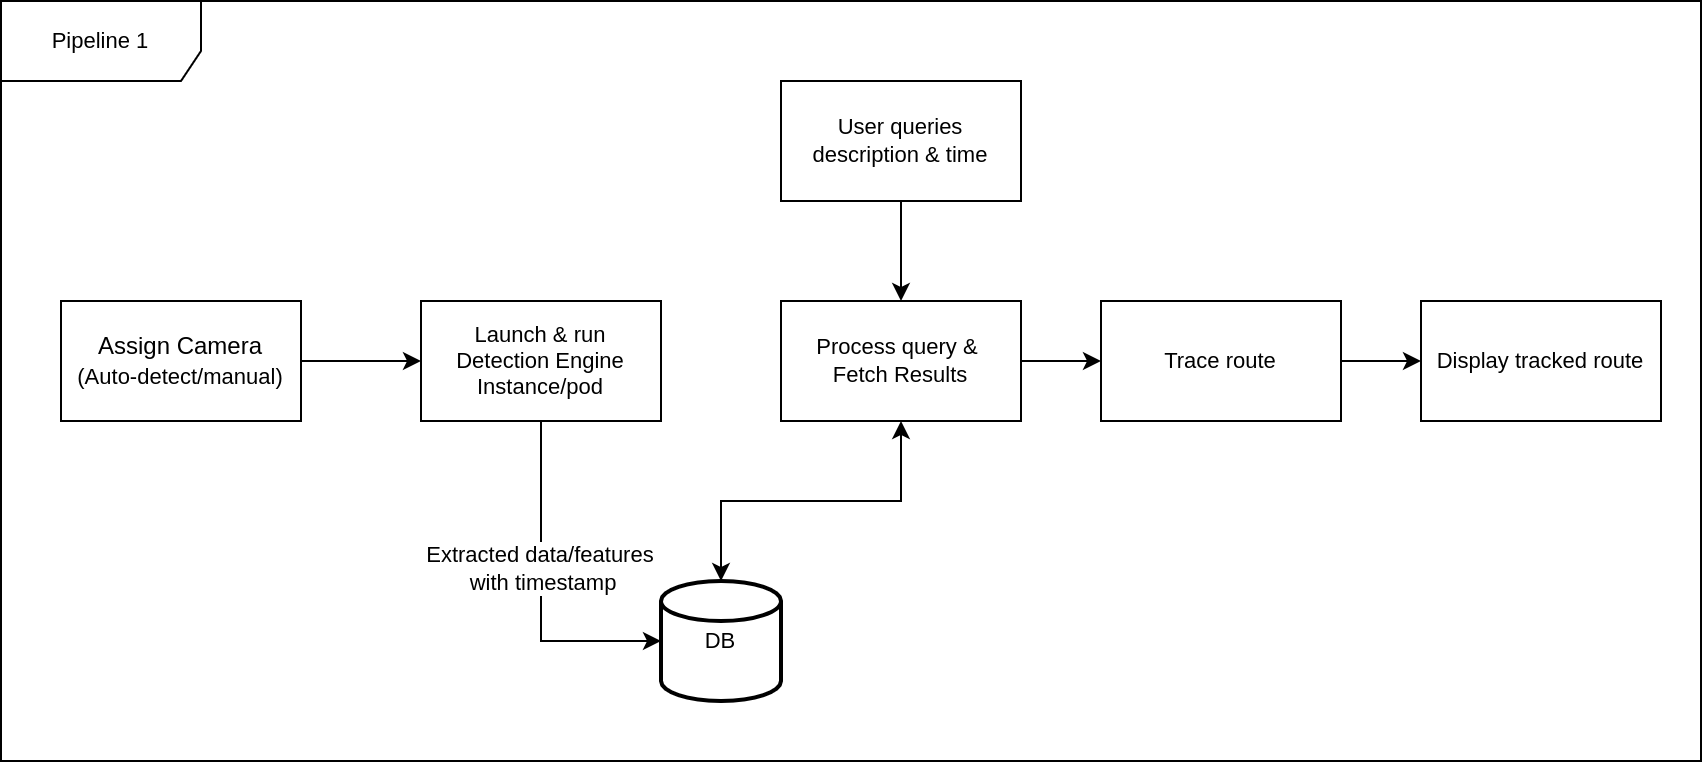
\includegraphics[width=0.95\textwidth]{res/pipeline1.png}
	\end{figure}
\end{frame}

\subsection{Detailed Design}
\begin{frame}{Detailed Design}
	\begin{figure}
		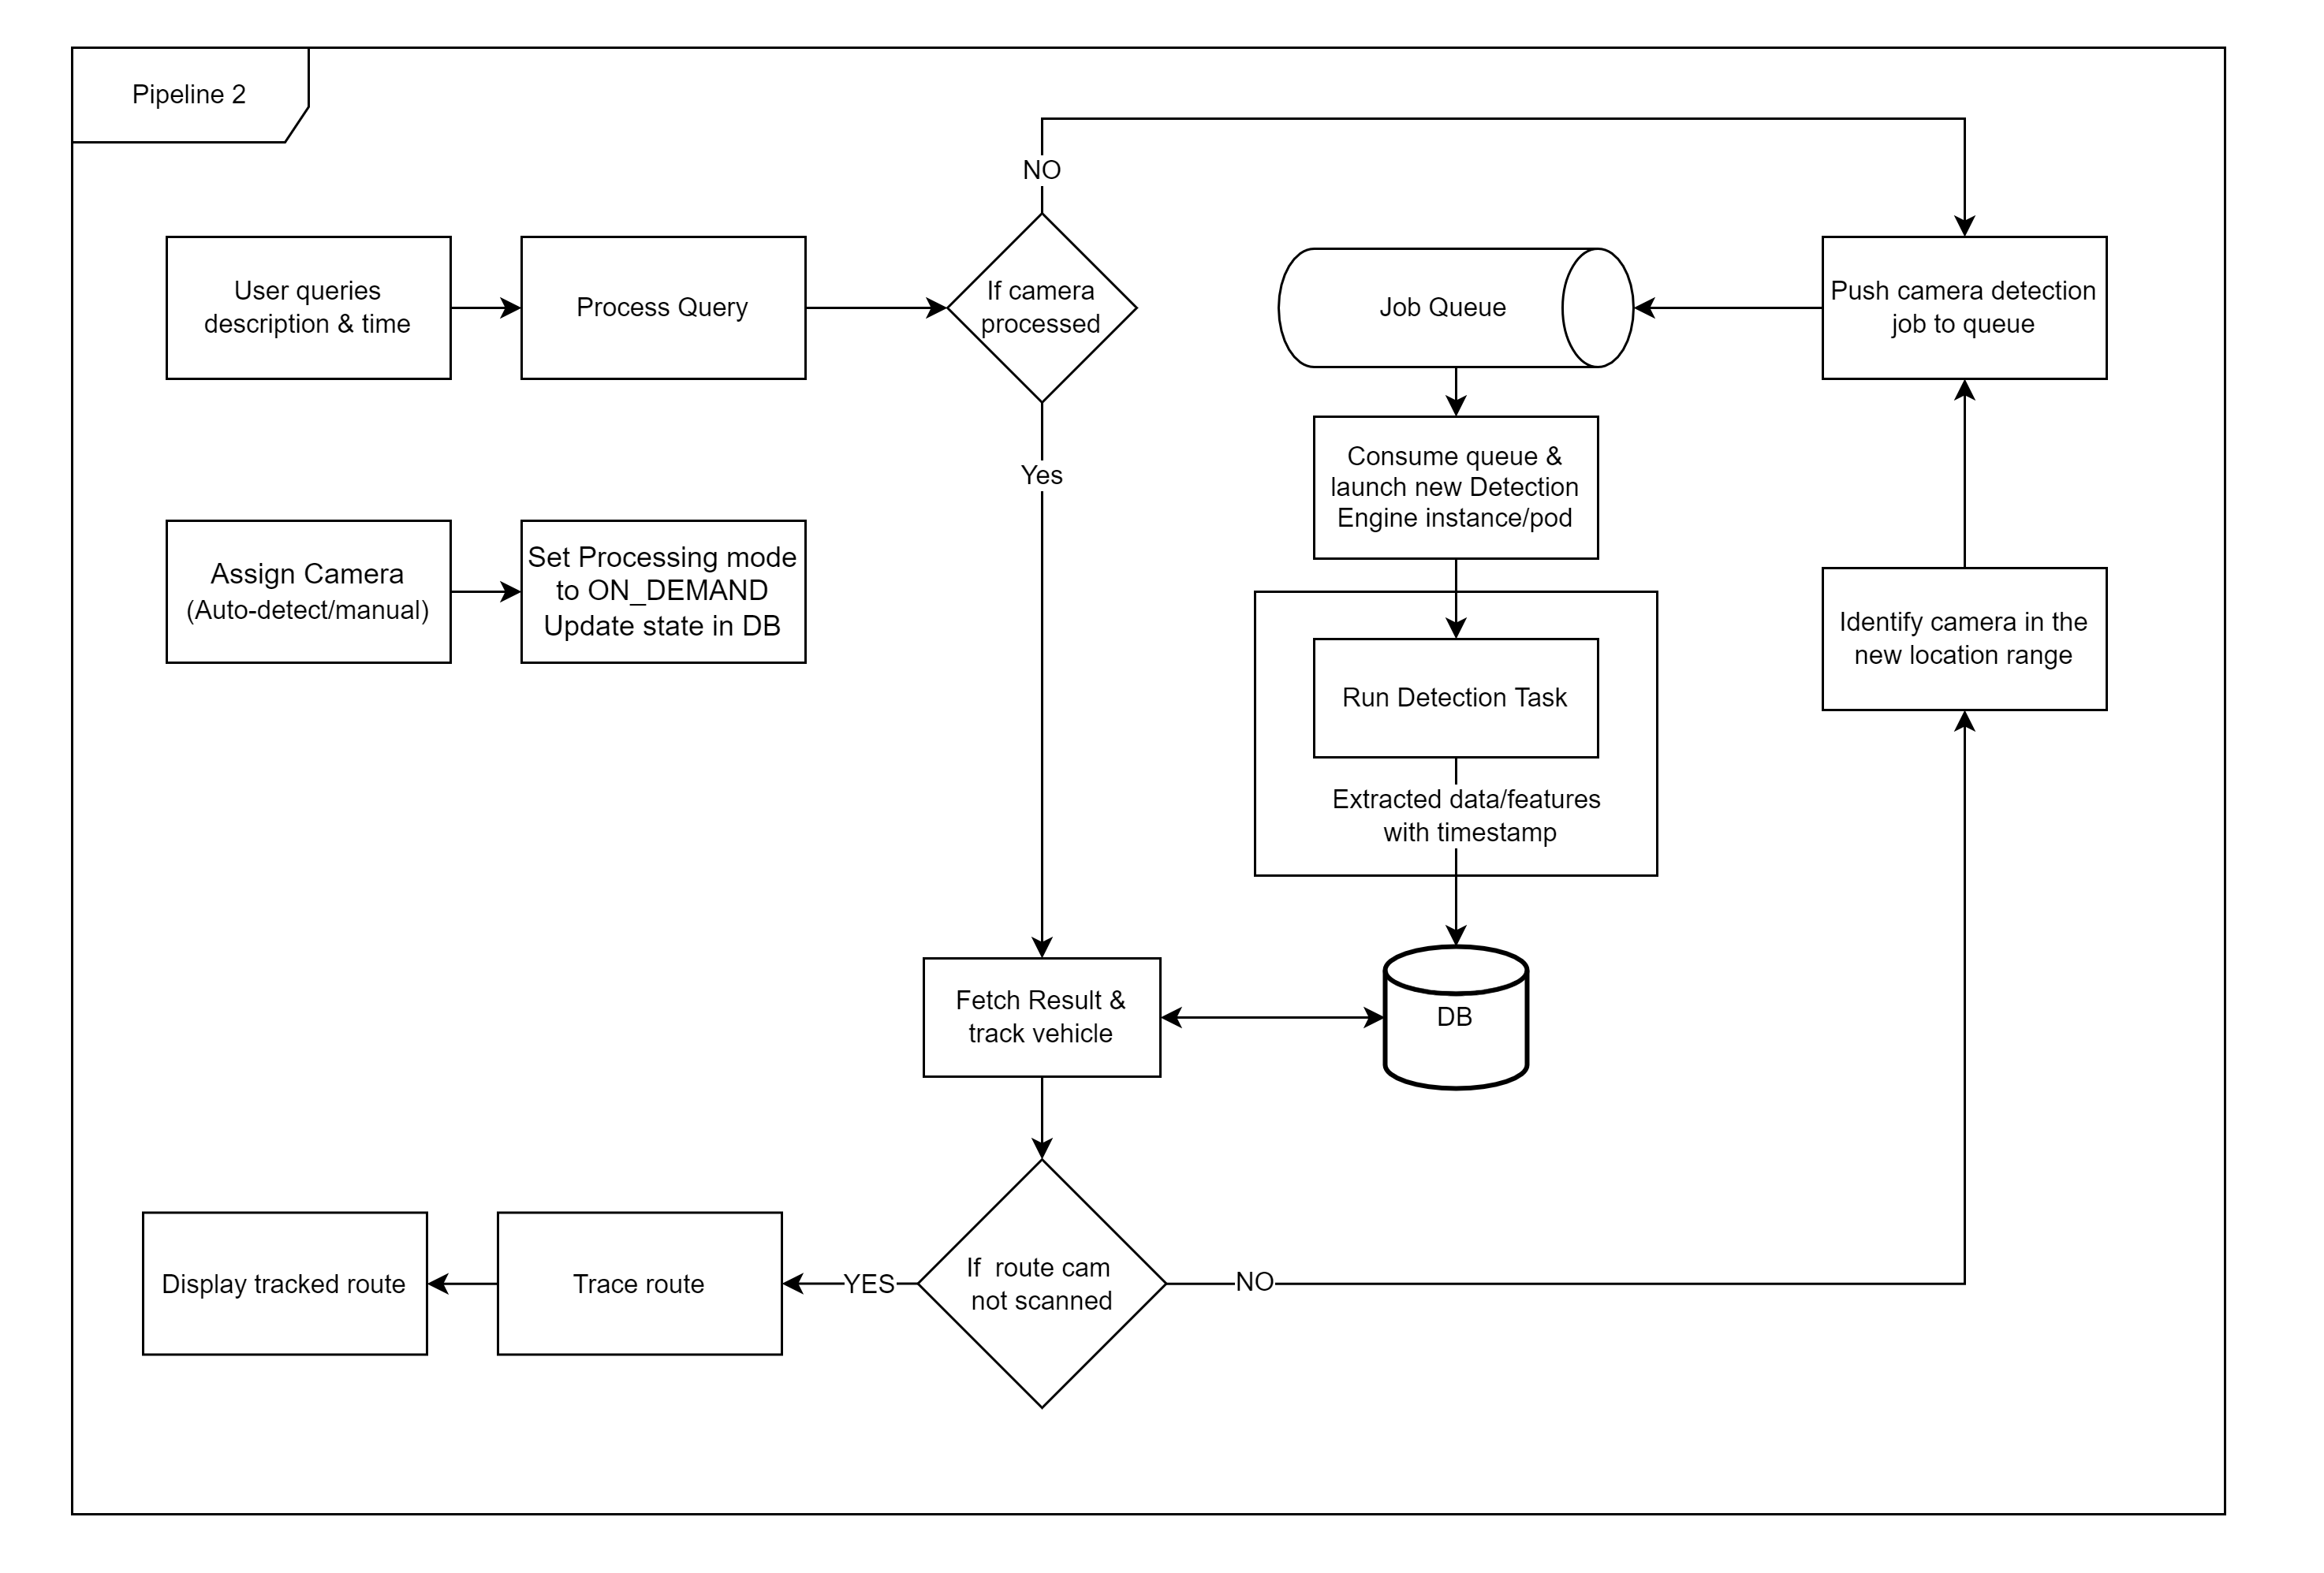
\includegraphics[height=0.8\textheight]{res/pipeline2.png}
	\end{figure}
\end{frame}

\subsection{Dataset}
\begin{frame}{Dataset}
	\begin{block}{Input}
		\begin{itemize}
			\item Video
			\item Query
		\end{itemize}
	\end{block}
	\begin{block}{Output}
		\begin{itemize}
			\item Vector points
			\item Map
		\end{itemize}
	\end{block}
\end{frame}

%########################################################################################

\section{Work done so far}
\begin{frame}{Work done so far}
\end{frame}

%########################################################################################

\section{Work planned}
\begin{frame}{Work Planned}
\end{frame}

%########################################################################################

\section{Conclusion}
\begin{frame}{Conclusion}
\end{frame}

%########################################################################################

\section{References}
\begin{frame}[allowframebreaks, noframenumbering]{References}
	\nocite{*}
	\bibliographystyle{IEEEtran}
	\bibliography{IEEEabrv,reference.bib}
\end{frame}

%########################################################################################

\end{document} 